\section{A deterministic finite reduction to simple graphs}
\label{sec:finite}

Fix an integer $K\ge2$, put $J=10K$, and make the effective parameter
choices in Proposition~\ref{prop:bit-gap}. Write $\Cost_\infty$ for its
cost, and put
\[
 W=\sum_{j=1}^4 b_j^{-1}.
\]
This is a positive rational constant depending only on $K$. The Gaussian
randomness will now be replaced by one finite rational distribution. We
retain the full joint distribution of the queried sign tables.

\subsection{Rational Gaussian sign tables}

Let $c,g\in\R^X$ and $\lambda\in\R^{\C}$ have independent standard
Gaussian coordinates. Define the two tables on $\C$
\begin{align*}
 T_0(z)&=\sgn\left(N^{-1/2}\sum_{x\in X}c_x(-1)^{z_x}\right),\\
 T_1(z)&=\sgn\left(N^{-1/2}\sum_{x\in X}(c_x+\sigma g_x)(-1)^{z_x}
                         +\eta\lambda_z\right).
\end{align*}
Their pair is a random element of a finite set of size
$2^{2|\C|}$. All four tests are deterministic functions of this pair and
their finite random choices. The first uses both tables. The second uses
the same $T_1$ for $B$ and $B'$. The third forces one entry of $T_1$ to the
two specified values. The fourth uses the same $T_1$ on the two outer
alphabets. Thus a single approximation of $(T_0,T_1)$ suffices.

\begin{lemma}[Effective finite comparisons]\label{lem:finite-game}
There is a deterministic construction, with all preliminary work depending
only on $K$, of a finite rational replacement for the four tests such that
\begin{equation}\label{eq:uniform-finite-error}
 \abs{\Cost_{\mathrm{fin}}(f)-\Cost_\infty(f)}<\frac12
 \qquad\text{for every collection of folded proof tables }f.
\end{equation}
Consequently its minimum cost is less than $9/2$ in the YES case, and every
proof has cost greater than $10K-1/2$ in the NO case. The rational
distribution replacing $(T_0,T_1)$ has a positive integer common
denominator depending only on $K$, computed by the construction.
\end{lemma}

\begin{proof}
We give a deterministic rational approximation with any prescribed rational
accuracy $0<\eps<1/4$. Set
\[
 d=2N+|\C|,\qquad S=2|\C|,\qquad A=2N+1.
\]
The $S$ unforced threshold inputs are linear forms in a vector
$Z\in\R^d$ of independent standard Gaussians. Each input for $T_0$ has
variance $1$, and each input for $T_1$ has variance
$1+\sigma^2+\eta^2$. Its coefficient vector has $\ell^1$ norm at most
\[
 (1+\sigma)\sqrt N+\eta\le A.
\]
These bounds do not require nonsingularity of the joint distribution of
the threshold inputs.

Choose an integer $T_G\ge1$ such that
\[
 d/T_G^2<\eps/4.
\]
The probability $\alpha$ that $Z\notin[-T_G,T_G]^d$ is at most $d/T_G^2$,
by the second-moment bound in each coordinate and a union bound. Partition
$[-T_G,T_G]$ into $L$ equal intervals of length $h=2T_G/L$, with rational
midpoints. Choose the integer $L$ large enough that
\begin{equation}\label{eq:gaussian-mesh-choice}
 SAh<\eps/4.
\end{equation}
Endpoint conventions for the intervals are immaterial to their Gaussian
masses. Rounding an interior vector to its cell midpoint changes any
threshold input by at most $Ah/2$. If the corresponding signs change,
the original threshold input has absolute value at most $Ah/2$.
A centered Gaussian of variance at least one has density at most one,
so the probability of this event for any one threshold is at most $Ah$.
The union bound over all $S$ thresholds is therefore at most $SAh$.
In particular, all unrounded ties have probability zero.

For completeness, this estimate can be combined with truncation without
losing control at the boundary. Couple $Z$ with a vector $Y$ as follows:
keep $Y=Z$ when $Z$ is in the cube, and otherwise draw $Y$ independently
from the Gaussian conditioned on the cube. Then $Y$ has exactly that
conditional law. On the event that $Z$ is outside, charge the full
probability $\alpha$; on its complement use the preceding sign-change
estimate. Hence the law of the original joint sign table and the law
obtained by rounding the conditioned Gaussian differ in total variation
by at most
\begin{equation}\label{eq:tail-and-grid-error}
 d/T_G^2+SAh<\eps/2.
\end{equation}

We next compute rational approximations to the conditioned Gaussian cell
masses, including their exact normalization. This step uses no real-number
oracle. Put $U=T_G^2/2$, and choose an integer $r\ge0$ such that
\[
 e_r:=\frac{U^{2r+1}}{(2r+1)!}
 \quad\text{satisfies}\quad 2dT_G e_r<\eps/4.
\]
This is a terminating search with rational comparisons. Indeed
$e_{r+1}/e_r=U^2/((2r+2)(2r+3))$, so after an effectively found index
the ratio is at most $1/2$. Define the rational polynomial
\[
 Q_r(v)=\sum_{j=0}^{2r}\frac{(-1)^jv^{2j}}{2^j j!}.
\]
Taylor's remainder for $e^{-u}$, with $u=v^2/2\ge0$, gives
\begin{equation}\label{eq:positive-density-polynomial}
 0\le Q_r(v)-e^{-v^2/2}\le e_r
 \qquad (|v|\le T_G).
\end{equation}
In particular $Q_r$ is strictly positive on the interval. For each grid
interval $I=[a,b]$, compute the rational number
\begin{equation}\label{eq:rational-cell-mass}
 w_I=\frac{\displaystyle\int_a^b Q_r(v)\dd v}
            {\displaystyle\int_{-T_G}^{T_G} Q_r(v)\dd v}.
\end{equation}
Both integrals are evaluated by the rational antiderivative
\[
 \sum_{j=0}^{2r}\frac{(-1)^jv^{2j+1}}{2^j j!(2j+1)}.
\]
Thus the $w_I$ are positive rationals and their sum is exactly one.

Here is a quantitative error bound for these cell masses. Write
$g(v)=e^{-v^2/2}$ on $[-T_G,T_G]$, let $Z_g=\int_{-T_G}^{T_G}g$, and let
$E_r=\int_{-T_G}^{T_G}(Q_r-g)$. Since $T_G\ge1$ and $e^{-u}\ge1-u$ for
$u\ge0$,
\[
 Z_g\ge\int_{-1}^1(1-v^2/2)\dd v>1,
 \qquad 0\le E_r\le2T_G e_r.
\]
The probability density $Q_r/(Z_g+E_r)$ is a mixture of $g/Z_g$ and
the normalized nonnegative residual $Q_r-g$, with residual mixture
weight $E_r/(Z_g+E_r)$ (if $E_r=0$ the densities coincide).
Their total variation distance is therefore at most $2T_G e_r$.
The Gaussian conditioned on the cube is a product of these
one-dimensional conditioned laws. Taking products increases the total
variation error by at most the sum of the coordinate errors, as follows
by replacing the coordinates one at a time. Rounding to the grid cannot
increase total variation. Consequently the grid distribution assigning
mass $\prod_{i=1}^d w_{I_i}$ to a cell has total variation distance at
most $2dT_G e_r<\eps/4$ from the rounded conditional Gaussian law.
Together with \eqref{eq:tail-and-grid-error}, this proves error less than
$\eps$ for the complete joint sign table.

Every sign at a rational midpoint is also computed exactly. A $T_0$
input has the sign of a rational number. Multiplying a $T_1$ input by
$\sqrt N>0$ expresses it as
\[
 a+b\sqrt N\qquad(a,b\in\mathbb Q).
\]
If $a,b$ have the same sign, or one is zero, its sign is immediate.
If their signs are opposite, compare the rationals $a^2$ and $Nb^2$;
the term of larger magnitude determines the sign, and equality is
an exact zero. Declare the sign of zero to be $+1$. This also handles
square $N$. Thus grid ties and all algebraic comparisons use finite
rational arithmetic.

Choose a common denominator $Q_1$ for the finitely many rationals $w_I$,
for example the product of their reduced positive denominators, and put
$Q=Q_1^d$. Every cell probability is an integer multiple of $1/Q$.
Enumerate the $L^d$ cells, compute their complete sign-table pairs, and
add the integer numerators for cells giving the same pair. This gives
an explicit rational law $\widehat\mu$ for $(T_0,T_1)$ with denominator
$Q$. The code $\C$, the grid, the polynomial, these numerators, and all
sign classifications are computed from the fixed parameters. Their
complete enumeration and the bit operations on their rational numbers
are finite work depending only on $K$ and $\eps$.

Finally take $\eps=1/(8(1+W))$. For each fixed outer sample and each
fixed collection of finite random choices in a test, its failure
indicator for any fixed proof is a function of the joint table with
values in $\{0,1\}$. Replacing its law by $\widehat\mu$ changes its
expectation by less than $\eps$. Averaging the finite choices and the
outer sample preserves this bound. It follows simultaneously for every
proof $f$ that
\[
 \abs{\Cost_{\mathrm{fin}}(f)-\Cost_\infty(f)}
 <\eps W<\frac12.
\]
No union bound over proofs is involved. Applying
Proposition~\ref{prop:bit-gap} gives the two claimed finite cost bounds.
\end{proof}

\subsection{Numerical multiplicities and canonical proof variables}

Let $M_0\ge1$ be the length of the uniform equation list from
Theorem~\ref{thm:max3lin}. The rounding needed to obtain that list was
included in its proof. Set
\[
 H_K=\binom{t}{t_0}3^{t_0},\qquad M=mn^{m-1}.
\]
There are exactly $H_KM_0^t$ elementary outer samples: ordered choices of
list entries, a hidden-coordinate set, and a position at every hidden
coordinate. Each has probability $1/(H_KM_0^t)$. For the first three
tests enumerate the full outer sample and ignore its unused information;
this gives exactly the required second-question marginal. Repeated
question encodings are identified as specified in Section~\ref{sec:outer}.
The sampling indices are not appended to actual questions.

All remaining probability denominators divide an effectively computable
integer $A_K$ depending only on $K$. An explicit choice can be given.
Write the row-resampling probability in lowest terms as
$\delta^2/m=a_0/r_0$, and use the Gaussian-table denominator $Q$ from
Lemma~\ref{lem:finite-game}. Each second alphabet has dimension at most
$3t$, so a uniform row in $D(A_V)$ has a probability denominator dividing
$2^{3t+1}$. Sample both the original and fresh replacement arrays even
when some or all replacement rows are unused, and similarly allow the
unused resampling flags and forced codeword to be drawn in every test.
Their joint probabilities have denominators dividing
\begin{equation}\label{eq:inner-denominator}
 A_K=Q\,2^{2M(3t+1)}r_0^M|\C|.
\end{equation}
Every elementary test outcome therefore has probability
$a/(H_K A_K M_0^t)$ for a nonnegative integer $a$. Dummy choices do not
change any test's distribution. They only give a uniform denominator.

Write $b_j=s_j/t_j$ in lowest terms, with positive integers $s_j,t_j$,
and choose a positive integer $B_K$ divisible by all four $s_j$.
The common denominator for the \emph{cost weights} can now be taken to be
\begin{equation}\label{eq:polynomial-denominator}
 D_0=C_KM_0^t,\qquad C_K=H_KA_KB_K.
\end{equation}
Indeed an elementary outcome of test $j$ contributes weight
$a t_j/(H_KA_KM_0^t s_j)$ times its failure indicator, and multiplication
by $D_0$ gives the integer $aB_Kt_j/s_j$. Zero multiplicities may be
omitted. Summing all multiplicities, before or after collecting equal
demands, gives exactly
\begin{equation}\label{eq:total-multiplicity}
 \sum_{\text{elementary demands}}\text{multiplicity}
 =D_0\sum_{j=1}^4b_j^{-1}=D_0W=O_K(M_0^t).
\end{equation}
This is a bound on their numerical sum, so expanding the multiplicities
is polynomial work for fixed $K$.

We describe explicitly the finite proof variables to which these demands
refer. Each $A_U$ is a nonempty affine subset of at most $3t$ bit slots,
and each $A_V$ has at most $3t$ slots. List each alphabet in lexicographic
order. Its affine forms can be found by binary Gaussian elimination and
enumerated by their truth tables; there are at most $2^{3t+1}$ forms.
Its Boolean query tables can all be enumerated as well, in number at
most $2^{2^{3t}}$. These are constants for fixed $K$. All pullbacks and
the arrays $B(x)$ are evaluated on these explicit tables. In particular,
the construction never computes a smoothed derivative, a Fourier decoder,
or an optimum proof.

For each actual question on each side, introduce one sign variable for
every complementary pair $\{P,-P\}$ of Boolean tables on its alphabet.
The two tables are distinct because the alphabet is nonempty. If $a_*$
is its first label, define
\[
 \tau(P)=P(a_*),\qquad R(P)=\tau(P)P.
\]
The representative $R(P)$ takes value $+1$ at $a_*$. Assigning a sign
$y_{q,R}\in\{-1,1\}$ to each such representative is in bijection with
folded proofs, by
\begin{equation}\label{eq:finite-folding}
 f_q(P)=\tau(P)y_{q,R(P)}.
\end{equation}
Here $q$ includes the first- or second-side tag and the actual question,
but no description of an outer-sample occurrence. Identical semantic
query tables at the same question therefore use the same variable.

A comparison $f_q(P)=f_{q'}(P')$ becomes the signed demand
\begin{equation}\label{eq:signed-demand}
 y_{q,R(P)}y_{q',R(P')}=\tau(P)\tau(P').
\end{equation}
The required relation is equality when the right side is $+1$ and
inequality when it is $-1$. This formula applies even when the two
variables coincide: a self-equality never fails and a self-inequality
always fails. Equation~\eqref{eq:finite-folding} proves exact equality
between weighted demand cost and $\Cost_{\mathrm{fin}}$, for every
assignment, including these cases.

\subsection{Exact realization by an unweighted simple graph}

\begin{lemma}[Path realization]\label{lem:graph-realization}
The finite rational comparison system can be transformed deterministically
into a simple undirected unweighted graph $G$ with
\begin{equation}\label{eq:exact-graph-optimum}
 \OPT_{\mathrm{uncut}}(G)
 =D_0\min_f\Cost_{\mathrm{fin}}(f).
\end{equation}
The graph has $O_K(M_0^t)$ vertices and edges and is constructed in
polynomial time, including bit complexity, for fixed $K$.
\end{lemma}

\begin{proof}
Start with a vertex for each sign variable. For every unit of integer
multiplicity in \eqref{eq:signed-demand}, join its endpoint vertices
by a path of length four for an equality demand and length three for an
inequality demand. See Figure~\ref{fig:paths}. All internal vertices are fresh for that unit demand.
If the two endpoints coincide, this prescription means respectively
a four-cycle through three fresh vertices or a triangle through two
fresh vertices.

\begin{figure}[htbp]
\centering
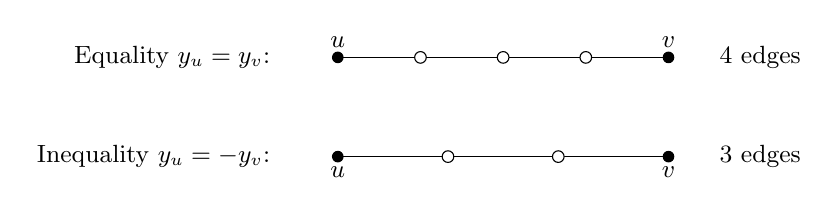
\begin{tikzpicture}[every node/.style={font=\small},scale=1.05]
\node[anchor=east] at (-.7,1.2) {Equality $y_u=y_v$:};
\node[anchor=east] at (-.7,0) {Inequality $y_u=-y_v$:};
\draw (0,1.2) -- (4,1.2);
\draw (0,0) -- (4,0);
\foreach \x in {0,4} {
 \fill (\x,1.2) circle (2pt);
 \fill (\x,0) circle (2pt);
}
\foreach \x in {1,2,3} \draw[fill=white] (\x,1.2) circle (2pt);
\foreach \x in {1.333,2.667} \draw[fill=white] (\x,0) circle (2pt);
\node[above] at (0,1.2) {$u$};
\node[above] at (4,1.2) {$v$};
\node[below] at (0,0) {$u$};
\node[below] at (4,0) {$v$};
\node[anchor=west] at (4.5,1.2) {$4$ edges};
\node[anchor=west] at (4.5,0) {$3$ edges};
\end{tikzpicture}

\caption{Each unit demand becomes a path with fresh internal vertices.
For fixed endpoint signs, its minimum uncut cost is zero if the demand
holds and one otherwise. Identifying the endpoints gives a four-cycle
or a triangle and handles self-demands with the same exact cost.}
\label{fig:paths}
\end{figure}


For an ordinary path with $L$ edges, write the vertex signs along it as
$x_0,\ldots,x_L$, and let $r$ be the number of its uncut edges.
Exactly $L-r$ adjacent pairs have opposite signs. Hence
\begin{equation}\label{eq:path-parity}
 x_0x_L=\prod_{i=1}^L x_{i-1}x_i=(-1)^{L-r}.
\end{equation}
When the prescribed relation holds, alternating signs from the first
endpoint give $r=0$ and reach the prescribed last sign. When it fails,
\eqref{eq:path-parity} rules out $r=0$; making exactly one adjacent
pair equal and alternating on all other edges reaches the prescribed
last sign and gives $r=1$. The same argument with $x_L=x_0$ proves
the assertion for coincident endpoints. A four-cycle has minimum zero,
as required by a self-equality; a triangle has minimum one, as required
by a self-inequality. Thus each gadget has conditional minimum equal
to the failure indicator of its demand.

For any fixed signs on the original vertices, its gadgets can attain
these minima independently because their internal vertices are disjoint.
Conversely any sign assignment on the graph pays at least the sum of
these conditional minima. Minimizing over the original signs and using
\eqref{eq:finite-folding} proves \eqref{eq:exact-graph-optimum}, with
no additive term.

No gadget has a loop or a repeated edge. Within a gadget all its internal
vertices are distinct; the coincident-endpoint cases have lengths at
least three. Between gadgets an edge cannot be repeated, since every
edge contains a vertex internal to its own gadget. The construction
therefore gives a simple undirected graph and assigns every edge unit
weight.

There are at most $2H_KM_0^t$ actual questions, and a constant number
depending only on $K$ of sign variables at each. A gadget introduces at
most three vertices and four edges. Equation~\eqref{eq:total-multiplicity}
therefore proves the stated size bound. All actual questions and query
tables can be identified by deterministic comparisons or sorting of
their canonical encodings. Equality of variable names, construction of
the affine alphabets, and table pullback require a polynomial amount of
work per outer sample; the only unbounded strings are names from the
polynomial-size starting instance. The sample count is polynomial for
fixed $t$. The integers in \eqref{eq:polynomial-denominator} and
\eqref{eq:total-multiplicity} have $O_K(1+\log M_0)$ bits. Explicitly
writing their multiplicities costs $O_K(M_0^t)$ iterations, and vertex
identifiers have $O_K(1+\log M_0)$ bits. These observations include the
cost of constructing the vertex and edge lists and all required integer
arithmetic.
\end{proof}

\subsection{The strict gap and algorithmic consequences}

\begin{proof}[Proof of Theorem~\ref{thm:main}]
Given a $3$SAT instance, perform the deterministic reduction in
Theorem~\ref{thm:max3lin} with the rational completeness error chosen by
Proposition~\ref{prop:bit-gap}. It supplies the nonempty uniform list of
length $M_0$. Carry out Lemmas~\ref{lem:finite-game} and
\ref{lem:graph-realization}, compute $D_0$ by
\eqref{eq:polynomial-denominator}, and output the graph together with
\[
 k=5D_0.
\]
This is a positive integer, computed without knowledge of the optimum.
In the YES case these Lemmas give
\[
 \OPT_{\mathrm{uncut}}(G)<\frac92D_0<5D_0=k.
\]
In the NO case they give
\[
 \OPT_{\mathrm{uncut}}(G)>
       \left(10K-\frac12\right)D_0
       >5KD_0=Kk,
\]
where the second inequality holds for every $K\ge2$.

All parameter searches in the preceding sections use the displayed
effective inequalities. The additional integer searches, rational
integrations, cell enumerations, and sign-table construction in this
Section are also algorithms. The reduction performs this preliminary
work itself; no table or numerical advice is supplied to it. Its cost
is a finite constant for fixed $K$. The starting reduction has
polynomial work and output length, and Lemma~\ref{lem:graph-realization}
establishes polynomial work and output length for every subsequent
step. The integer $k$ has $O_K(1+\log M_0)$ bits. Composition is
therefore a deterministic polynomial-time many-one reduction with all
the graph properties and the strict positive-threshold gap in the
statement.
\end{proof}

For clarity, the deterministic and randomized approximation consequences
are distinct. Let $C>1$ be a fixed real factor and choose a fixed integer
$K\ge\max\{2,C\}$. A deterministic polynomial-time algorithm returning
a bipartition of cost at most $C\OPT_{\mathrm{uncut}}(G)$ would decide
$3$SAT: run it on the output graph and accept exactly when its cut has
cost at most $Kk$. In a YES instance its cost is at most $Ck\le Kk$;
in a NO instance every bipartition costs more than $Kk$. Thus such an
algorithm implies $\mathsf P=\NP$.

If instead a randomized polynomial-time algorithm returns such a
bipartition with probability at least a fixed positive constant, validate
the returned bipartition and apply the same cost check. A NO instance
can never be accepted, regardless of the algorithm's random choices.
A YES instance is accepted whenever the approximation succeeds.
Independent repetition a fixed number of times raises this probability
to at least $1/2$ if necessary. This puts $3$SAT in $\RP$, and composing
with deterministic reductions to $3$SAT gives $\NP\subseteq\RP$.
The randomized conclusion is therefore the latter containment.

\subsection{Minimum 2CNF clause deletion}
\label{sec:2cnf-consequence}

\begin{proof}[Proof of Corollary~\ref{cor:min-2cnf-deletion}]
Given $G=(V,E)$, introduce a variable $x_v$ for each vertex and, for each edge
$uv$, the two clauses
\[
 (x_u\lor x_v),\qquad(\neg x_u\lor\neg x_v).
\]
Call the resulting formula $F_G$. Equal endpoint values falsify exactly one
of these clauses, while unequal values satisfy both. Thus, for every
assignment $a$ and $S_a=\{v:a(x_v)=1\}$,
\[
 \operatorname{unsat}(F_G,a)=\Uncut_G(S_a).
\]
Deleting an assignment's false clauses gives a feasible deletion set of the
same cost. Conversely, from every feasible deletion set $D$, a polynomial-time
$2$SAT algorithm finds an assignment $a$ satisfying $F_G\setminus D$.
Every original clause it falsifies belongs to $D$, so
$\Uncut_G(S_a)=\operatorname{unsat}(F_G,a)\le\abs{D}$. Consequently,
\[
 \OPT_{\rm del}(F_G)=\min_a\operatorname{unsat}(F_G,a)
                  =\OPT_{\rm uncut}(G).
\]

Fix $C>1$ and choose a fixed integer $K\ge\max\{2,C\}$ in
Theorem~\ref{thm:main}. The construction has $\abs{V}$ variables and
$2\abs{E}$ clauses and preserves the gap at the same binary-encoded integer
$k\ge1$: $\OPT_{\rm del}(F_G)\le k$ if the source formula is satisfiable,
and $\OPT_{\rm del}(F_G)>Kk$ otherwise. A $C$-approximation
returns a feasible deletion set with $\abs{D}\le Ck\le Kk$ in the former
case, whereas every feasible deletion set has $\abs{D}>Kk$ in the latter.
Comparing its size with the integer $Kk$ therefore decides $3$SAT in
polynomial time.
\end{proof}
